\chapter{Development of a device for direct counting of the number of particles in the beam}

\section{Introduction}
This chapter will focus on the devices used within the MoVe\_IT project in order to obtain a single proton counting device.
This comprehends the solid state detector, the ASICs used to digitalise the signal and the final read-out board.
\begin{figure}[H]
	\centering
	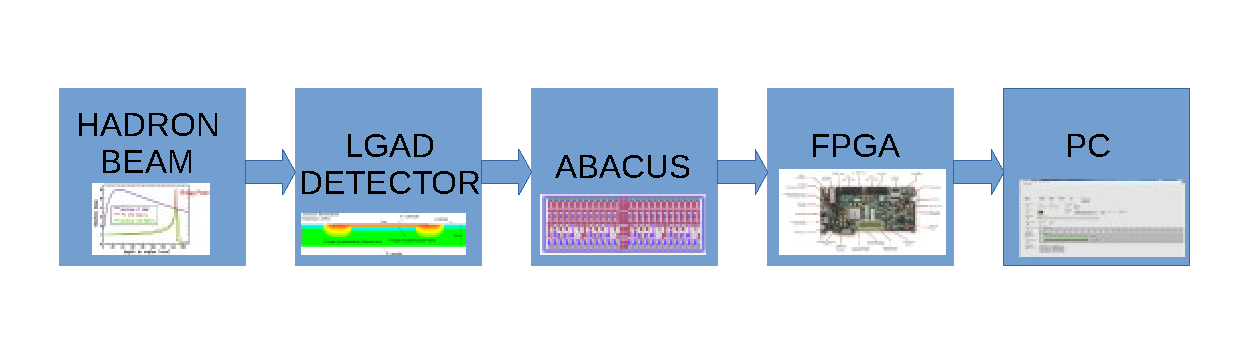
\includegraphics[width=0.99\linewidth]{IMG/ch2/BLOCK}
	\caption{Data flow, from beam to pc}
	\label{fig:block}
\end{figure}
\noindent In figure \ref{fig:block} it can be seen a diagram with the "data flow" of the Project.
The particle beam coming from the accelerators are detected by a LGAD (Low Gain Avalanche Diode) sensor that will be discussed in section \ref{lgad}, the current signal coming from the detector is the digitalized by the second version of a full custom circuit called ABACUS\_v2 that will be discussed in section \ref{chip}.
This ASIC will be mounted on a full custom PCB named EsaAbacus that will be analysed in section \ref{esaabacus}.
The data from the chip is then read by an FPGA board, a general purpose device that will be analysed in detail within chapter 3.
The FPGA elaborates the data and finally sends them to a computer. In the final operational device the computer, on the base of the counted particles, should move and control the beam in a close and controlled loop. 

\section{MoVe\_IT project}\label{moveit}
\begin{figure}[H]
	\centering
	
\includegraphics[width=0.35\linewidth]{IMG/ch2/Move_IT_logo}
	%\caption{}
	%\label{fig:moveit}
\end{figure}
\noindent Currently the Medical Physics group at University of Torino and INFN (the Italian National Institute for
Nuclear and Particle Physics) is participating to the MoVe\_IT\cite{moveit} (Modeling and Verification for Ion beam Treatment planning)
research project, which aims to develop new and
innovative models for biologically optimized Treatment Planning Systems (TPS) using ion beams in hadron therapy.
As~part of the project the Torino group is involved in the development of solid state detectors and readout electronics for measuring with high precision
the characteristics of the hadron beam for irradiation, such as number of particles delivered per unit time, energy and beam profile.
The final goal is to prove the ability of LGAD detectors to discriminate individual protons and to count their number up to fluxes of 100~MHz/cm$^2$ with an uncertainty of less than 1\% which is the clinical tolerance required.
In order to do that a custom detector was built ad hoc for this purpose. It is a LGAD type sensor with an area of $\approx$ 3x3~cm$^2$ and 144 strips. It has a thickness of the active region of 50~$\mu$m.
The final goal is to use two of this sensors in orthogonal directions in order to obtain a greater spatial resolution.
A strip detector is limited in the maximum flux that can be monitored with accuracy, however it is useful in radiobiological experiments, for which it is not needed to reach therapeutic fluxes and often laterally spread-out beams are used\cite{hammad}.
The main key-points of the final design are:
\begin{itemize}
	\item A cover area of $\approx$ 3x3~cm$^2$
	\item A maximum measurable flux of 10$^8$~$\frac{p}{s \cdot cm^2}$ with less than 1\% error
	\item Sensitivity of single particle at low fluxes
	\item Provide beam shape in two orthogonal directions
\end{itemize}


\section{Low Gain Avalanche Diode (LGAD)}\label{lgad}
\noindent The first device involved is the detector. In order to be able to detect a single particle and to reduce the pile-up effects (that have been discussed with great detail in Limardi's masters degree thesis\cite{limardi}) short signals are mandatory. To obtain a short signal the active region of the sensor needs to be the as thin as possible. However the thinner the detector is the lower is the SNR (Signal to Noise Ratio).
To solve this problem the INFN decided to use a new type of sensors known as LGAD.
\noindent Low-Gain Avalanche Detectors (LGADs) are innovative detectors developed in collaboration with the Fondazione Bruno Kessler (FBK, Trento) which feature a moderate ($\approx$10) internal charge multiplication achieved through an additional p+ doping layer few microns depth. The increase signal-to-noise ratio allows designing very thin Ultra Fast Silicon Detectors (UFSD) designed for fast signal collection times, high rates and very good time resolution\cite{lgad}.
%%%%%%%%%%%%%%%%%%%%%%%%%%%%%%%%%%%%%%%%%%%%%%%%%%%%%%%%%%%%%%%%%%%%%%%%%%%%%%%%%%%%%%%%%%%%%%%%%%%%%%%%%%%%%%%%%
The basic doping profiles of the LGAD structure, based on a standard PIN detector, is shown in
figure \ref{fig:ufsdlgad}, showing a n++/p+/p/p++ structure.
The figure shows a highly doped n++ cathode electrode with a moderately doped p+ type region
below, known as the multiplication implant. The n-type electrode has a peak doping concentration
of order 1 $\cdot$ 10$^{19}$ cm$^{-3}$ and has a shallow profile into the bulk of $\approx$ 1 $\mu$m.
The p-type multiplication implant has a peak doping concentration of order 1 $\cdot$ 10$^{16}$ cm$^{-3}$
and has a significantly deeper profile into the bulk ($\approx$ 4 $\mu$m) than the n++ electrode. The bulk
material is high resistivity p-type silicon (approximately 10 k$\Omega$/cm) with a p++ anode electrode
on the backside.
\begin{figure}[H]
	\centering
	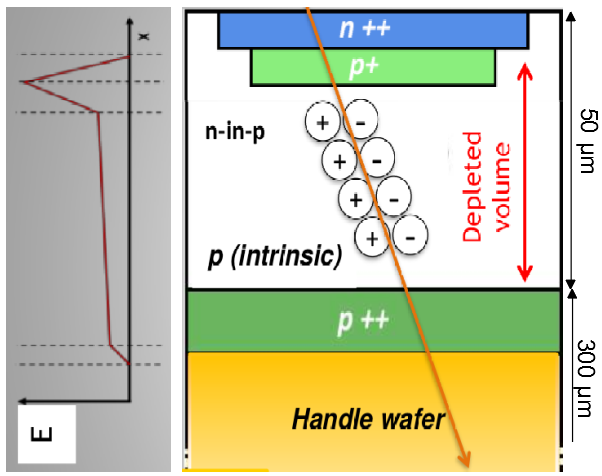
\includegraphics[width=0.35\linewidth]{IMG/ch2/UFSDLGAD.png}
	\caption{Schematic cross-section of the LGAD pad design. A p+ type layer is diffused below the n++ electrode to form the n++/p+/p junction where the multiplication takes place}
	\label{fig:ufsdlgad}
\end{figure}
\noindent The LGAD device is operated with the bulk over depleted. Incident radiation produces electron-hole
pairs in the detector with drift towards the cathode and anode respectively. The maximum
electric field in the device is between the n++ cathode and the p+ type multiplication electrode and is
proportional to the square root of the p+ type doping density and proportional to the square root of the
external bias voltage for an abrupt junction approximation.
The radiation induced electrons in the detector cross this high field region. For sufficiently
high electric fields impact ionisation occurs which results in multiplication of the carriers and a
signal gain.
Increasing the high-field (either due to an increase in the doping density or
an increase in the external bias voltage) will increase the electron-hole pair generation rate. For a
low gain device, the desire is to have an overall gain of 10 at $\approx$~200~V bias, with a breakdown voltage
significantly higher than this at least $\approx$~400~V.
%%%%%%%%%%%%%%%%%%%%%%%%%%%%%%%%%%%%%%%%%%%%%%%%%%%%%%%%%%%%%%%%%%%%%%%%%%%%%%%%%%%%%%%%%%%%%%%%%%%%%%%%%%%%%%%%%
\begin{figure}[H]
	\centering
	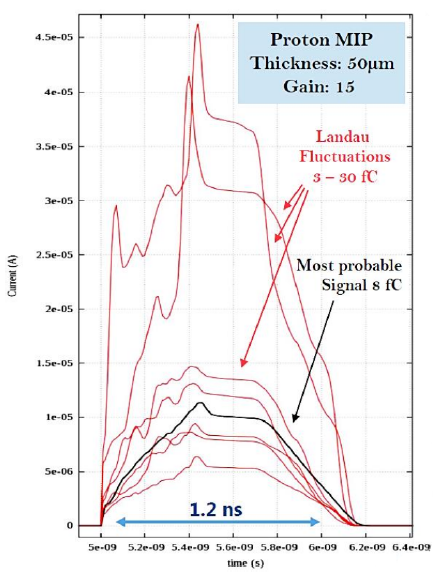
\includegraphics[width=0.35\linewidth]{IMG/ch2/LGAD_Signal}
	\caption{Simulated detector signal}
	\label{fig:signal}
\end{figure}
\noindent The output signal from a detector used in the project has a trapezoidal form, a duration of $\approx$ 1.2~ns (rise and fall times of $\approx$~450~ps and a 
flat region of $\approx$~300~ps) and a current in the order of 1$\cdot$10$^{/5}$~A.
In figure \ref{fig:signal} can be seen a signal simulation, the most probable signal carry a 8~fC charge, however due to the Landau Fluctuations this value can change between 3~fC and 30~fC.
%%%%%%%%%%%%%%%%%%%%%%%%%%%%%%%%%%%%%%%%%%%%%%%%%%%%%%%%%%%%%%%%%%%%%%%%%%%%%%%%%%%%%%%%%%%%%%%%%%%%%%%%%%%%%%%%%
\noindent The main risk in
the use of LGAD silicon detectors for beam monitoring is related to the high radiation doses from
therapeutic beams. The design of LGAD sensors has not been optimized yet for radiation
resistance, and the measurements performed up to now indicate a stable behavior up to 1014~n$_{eq}$/cm$^2$ for 300~$\mu$m thick detectors (this corresponds to a few hours of a therapeutical proton
pencil beam with an current of 1~nA and a FWHM of $\approx$ 1~cm); at higher doses the internal gain
of the sensors decreases and it is necessary to raise the bias voltage to keep a stable signal level.
It is expected that the use of thinner sensors (50~$\mu$m thickness) will decrease the trapping
probability in the sensors, therefore extending the operative time. Intense work is currently going
on in the LGAD community to increase the radiation resistance of the sensors. Several
approaches as alternative dopants and doping profiles are being investigated with the expectation
to reach a stable behavior up to >1015~n$_{eq}$/cm$^2$ fluencies in the next 1 or 2 years.


\section{ABACUS\_v2 chip}\label{chip}
\noindent The signal from figure \ref{fig:signal} of each detector strip is connected to an input channel of the new ABACUS\_v2 full custom chip\cite{abacus}\cite{dac} designed by the Turin INFN group and submitted on October 26$^{th}$ 2020.
\begin{figure}[H]
	\centering
	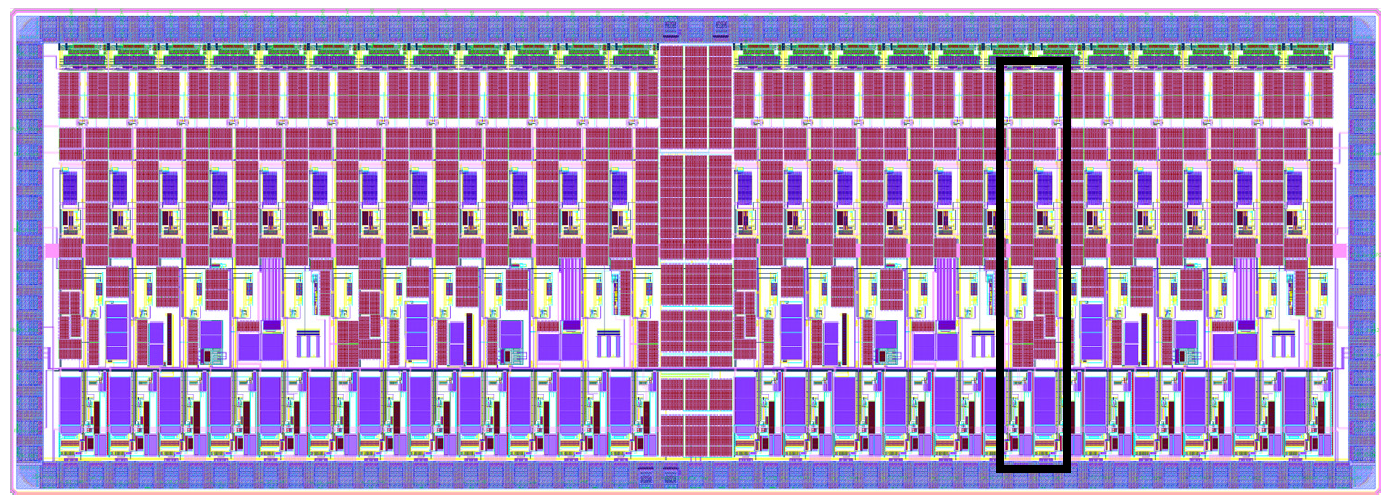
\includegraphics[width=0.9\linewidth]{IMG/ch2/ABACUS2.png}
	\caption{ABACUS\_v2 chip die view}
	\label{fig:abacus2}
\end{figure}
\noindent In figure \ref{fig:abacus2} it can be seen a schematic of the chip die area. Inside the black rectangle it can be seen a single channel. Its design will be analysed later in this section.
This prototype is a 24 channels ASIC designed in UMC (United Microelectronics Corporation) 110~nm technology.
The die size is 4.95~x~1.935~mm$^2$.
The 24 channels are divided in two 12-channels groups. The two groups differs for the architecture of the first stage only.
The first group (group A) is based on a TIA (Trans-Impedance Amplifier) architecture with a two stage core amplifier.
The second group (group B) is based on a Regulated Common Gate (RCG) input stage followed by a single stage TIA.
The pro and cons of the two architectures will not be a part of this thesis.\\
As already discussed, the design goal of the counting device is to measure the number of protons with a maximum error of 1\% up to a fluxes of 10$^8$~p/(cm$^2$$\cdot$s).
For a single particle the efficiency must be greater than 99\%, and this defines the range of charges the electronics must be able to accept.
The ABACUS\_v2 chip was optimized for an input capacitance between 5 and 20 pF and to cope with continuous signals up to 100 MHz rate.
It can accept input charges from 3~fC to 140~fC, has a dead time <~10~ns and a SNR~>~10. 

\subsection{ABACUS\_v2 Channel structure}
In order to understand the measurements from chapter 5 and the goal of this thesis work it is extremely important to analyse how the ABACUS\_v2 channel works.
In figure \ref{fig:abacuschannel} the block diagram of one channel is shown.
\begin{figure}[H]
	\centering
	\includegraphics[width=0.8\linewidth]{IMG/ch2/Abacus_channel.png}
	\caption{Single channel diagram of the ABACUS\_v2 chip}
	\label{fig:abacuschannel}
\end{figure}
\noindent A low noise CSA (Charge Sensitive Amplifier) (1) is followed by a low-pass filter (2).
The output signal from (2) has two components, a DC one, that is called Pedestal, and the actual amplified signal; this will be explained with more details in section \ref{considerations}.
The amplified signal is therefore fed to a leading-edge multistage discriminator (3 and 4) followed by a driver (5 and 6) which provides a logic pulse in Current Mode Logic (CML) format.
The output of the discriminator is also used in a feedback circuit (7 and 8) to reset the CSA feedback capacitance. This feedback circuit was designed for a fast baseline restoring and to avoid signal saturation (fast-reset signal).
The chip was heavily tested by INFN expertises; the output voltage from the amplifier and the noise were estimated by the measurement of the number of detected pulses as a function of the threshold value. The results are shown in figure \ref{fig:abacustest} for charges between 3 fC and 20 fC (measurement and analysis carried out by PhD \textit{Omar Hammad Ali}).
\begin{figure}[H]
	\centering
	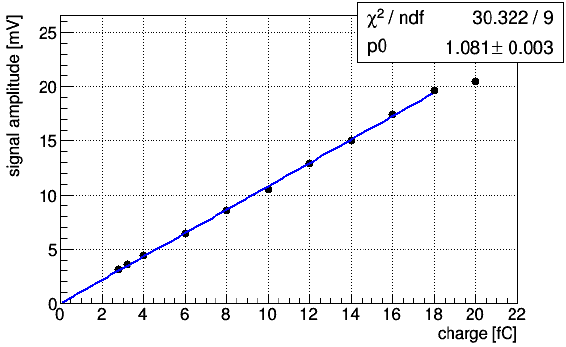
\includegraphics[width=0.6\linewidth]{IMG/ch2/ABACUSTEST}
	\caption{Amplitude of the amplifier output signal as a function of the charge injected at 1 MHz rate}
	\label{fig:abacustest}
\end{figure}
\noindent The most important considerations concern the functioning of the discriminator (3).
The threshold voltage (V$_{th}$) is the sum of two different components that are independently configurable:
\begin{itemize}
	\item An external 16~bit DAC (Digital to Analog Converter) for the global V$_{th}$ 
	\item A per channel programmable 6~bit internal DAC for threshold tuning
\end{itemize}
\noindent The main external DAC provides the same threshold voltage for every channel, however due to manufacturing tolerances not every channel is the same. One may have a slightly higher or lower input capacitance, or the amplifier could have a extremely low, but measurable, difference in gain.    
These inequalities may have a relevant impact on the measured particle rate, and thus on the dose given to the patient.
In order to reduce these differences each channel has an independently programmable 6~bit DAC that is used to fine-tune (trim) the V$_{th}$ value.    
\subsubsection{External DAC}
The external DAC is a commercially available Linear Technology LTC2604 Quad 16-bit Rail-to-Rail DAC.
The device uses the $I^2C$ protocol and reads 24~bit words configured as in figure \ref{fig:extdactiming2}, more details are provided in the data-sheet \cite{LTC2604}.
The main features are:
\begin{itemize}
	\item A guaranteed 16~Bit Monotonic Over Temperature
	\item An ultra-low Cross-talk Between DACs (<~5~$\mu$V)
	\item Separate Reference Inputs for each DAC
	\item Wide 2.5~V to 5.5~V Supply Range
	\item Low Power Operation: 250~$\mu$A per DAC at 3~V
\end{itemize} 
\begin{figure}[H]
	\centering
	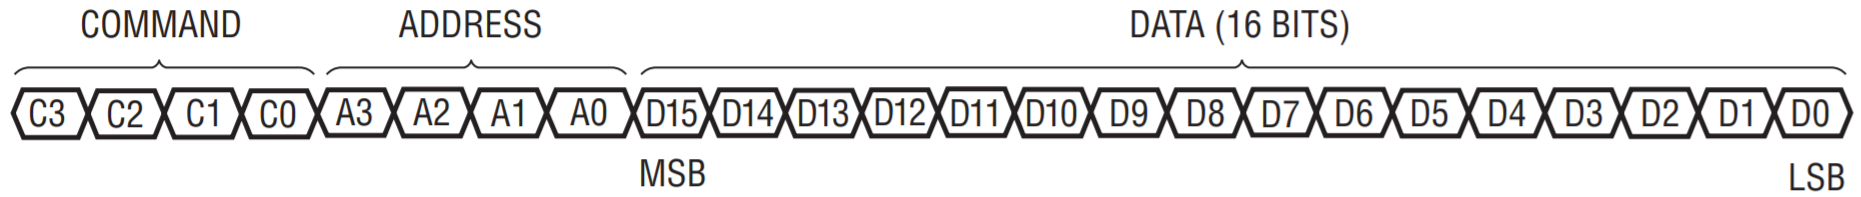
\includegraphics[width=0.99\linewidth]{IMG/ch2/EXTDACTIMING2}
	\caption{24~bit data sequence for the LTC2604 external DAC}
	\label{fig:extdactiming2}
\end{figure}
\subsubsection{Internal (Trimming) DAC}
The internal (Trimming) DACs, also called Baseline DACs in some papers, were designed specifically for this chip. Inside the die there is an $I^2C$ controller used to enable the communication between DAC and the world.
The DACs are programmed using 16~bit serial words; the configuration process is explained in detail in section \ref{InternalDac}.
\begin{figure}[H]
	\centering
	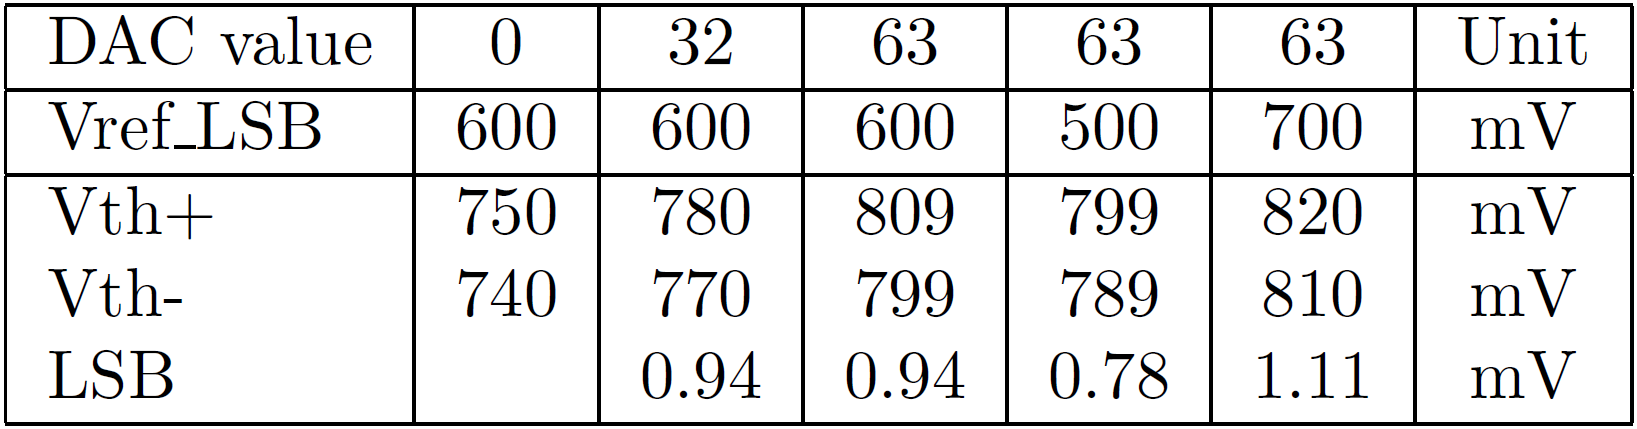
\includegraphics[width=0.5\linewidth]{IMG/ch2/INTDACTABLE}
	\caption{Internal DACs LSB values at different V$_{refLSB}$ settings}
	\label{fig:intdactable}
\end{figure}
\noindent In figure \ref{fig:intdactable} it can be seen that with a reference voltage of 600~mV the LSB should be 0.94~mV, this means that, being this a 6~bit DAC, the maximum trimming voltage is $\approx$~59.2~mV. For reference, an usual value for the pedestal voltage in around $\approx$~560~mV. Thus these internal DACs are used to fine tune the threshold voltage of the discriminator, while the bulk of the work is done by the external one.   

\section{ESA-ABACUS}\label{esaabacus}
\noindent As explained in section \ref{moveit} the final detector will have 144 strips, however each ABACUS\_v2 chip can read only 24 channels, this means that for the ultimate sensor read-out 6 chips are needed (24$\cdot$6~=~144).
In order to utilize these device at the same time the Turin INFN group developed, built and tested a new board, called ESA-ABACUS, that can accommodate and handle 6 ABACUS\_v2 chips. The ESA-ABACUS board can be seen in figure \ref{fig:esaabacus}.
\begin{figure}[H]
	\centering
	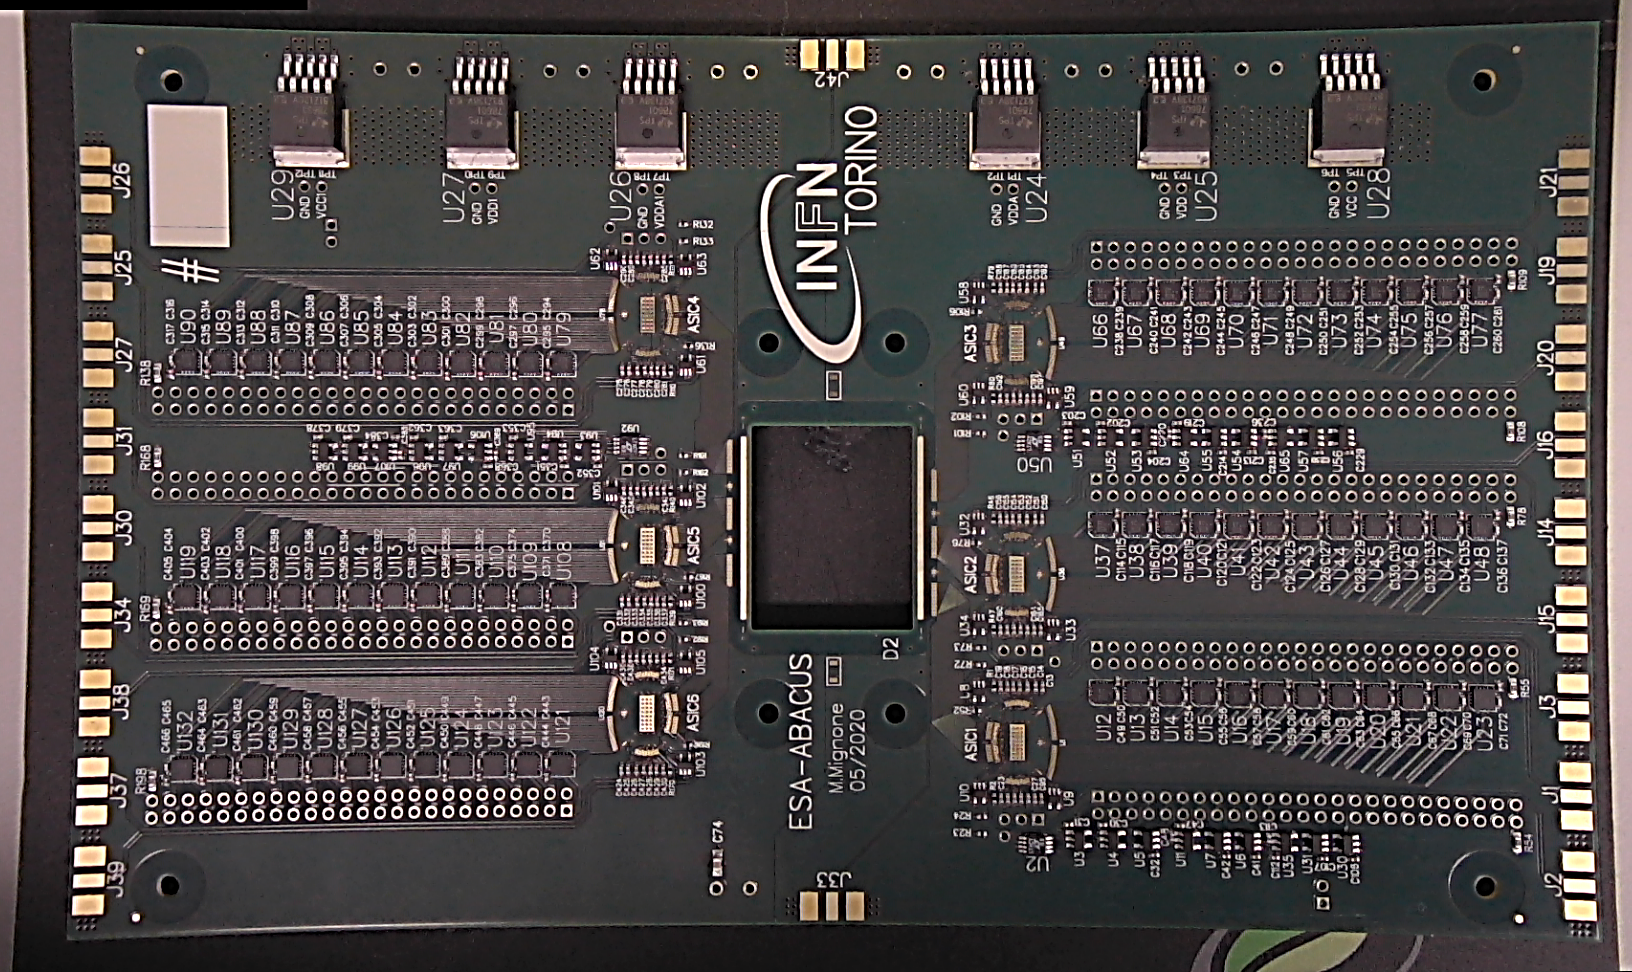
\includegraphics[width=0.7\linewidth]{IMG/ch2/EsaAbacus.png}
	\caption{Esa-Abacus board, chips and detector are not yet bonded}
	\label{fig:esaabacus}
\end{figure}
\noindent To be noted that each FPGA board used has enough Input/Output resources for two ABACUS\_v2 chips, this means that in order to utilize at his full potential the ESA-ABACUS three FPGA boards are needed (chapter 3 will explain in detail what an FPGA is).
The final goal is to use two of these devices placed in an orthogonal way in order to acquire the horizontal and vertical dispersion of the particle beam.
To be noted that this board, on the contrary of the ABACUS\_v2 test board that will be described in section \ref{testboard}, is not intended for the validation of the chip, in fact it has no trimmers for any voltage regulation, instead it was made in order to test and utilize the 144 strip detector.



\section{FPGA board tasks}
















